%%externalize tikz
%\usetikzlibrary{external}
%\tikzexternalize[prefix=licht/tikz/, figure name=plot]
%
%%used for drawing n(r)-Area
%\definecolor{lGray}{gray}{0.8}
%\definecolor{llGray}{gray}{0.9}
%\usepgfplotslibrary{fillbetween}
%
%\tikzset{
%  ring shading/.code args={from #1 at #2 to #3 at #4}{
%    \def\colin{#1}
%    \def\radin{#2}
%    \def\colout{#3}
%    \def\radout{#4}
%    \pgfmathsetmacro{\proportion}{\radin/\radout}
%    \pgfmathsetmacro{\outer}{.8818cm}
%    \pgfmathsetmacro{\inner}{.8818cm*\proportion}
%    \pgfmathsetmacro{\innerlow}{\inner-0.01pt}
%    \pgfdeclareradialshading{ring}{\pgfpoint{0cm}{0cm}}%
%    {
%      color(0pt)=(white);
%      color(\innerlow)=(white);
%      color(\inner)=(#1);
%      color(\outer)=(#3)
%    }
%    \pgfkeysalso{/tikz/shading=ring}
%  },
%}

%\usepackage{subcaption}
%\usepackage{subfigure}
    
\chapter{Lichtbrechung in der Atmosph"are\label{chapter:licht}}
\lhead{Lichtbrechung in der Atmosph"are}
\begin{refsection}
\chapterauthor{Simon Schaefer und Tibor Schneider}

%polar plot
\usepgfplotslibrary{polar}

\section{Einleitung}
\rhead{Einleitung}

Der Blick an den Nachthimmel fasziniert uns Menschen schon seit Jahrtausenden. "Ahnlich der Frage "uber das Leben nach dem Tod wurden damit ganze Religionen und Kulturen begr"undet beziehungsweise zugrunde gerichtet. 
"Uber die Jahrhunderte wuchs die Einsicht, wenn auch nicht stetig und leider auch nicht strikt monoton, dass eine genauere Vermessung des Nachthimmels, die Astrometrie, physikalische Grundlagen zur Diskussion beitragen kann. 


Schon Galileo Galilei beobachtete mit seinem Teleskop den Nachthimmel um seine Aussagen über die Bewegung der Erde um die Sonne zu belegen.
Er beobachtete die Bewegungen der Planeten unseres Sonnensystems und nahm die Positionen, Grössen und den Abstand entfernter Sterne, Galaxien und anderen Objekten als sogenannte Fixsterne konstant an. 
W"ahrend die NASA und andere noch daran t"ufteln, einen Menschen auf unseren n"achsten Nachbarplaneten zu bugsieren, sind unsere Blicke und vor allem unsere Neugier bereits Milliarden von Lichtjahren "uber unser Sonnensystem hinaus ins Weltall gerichtet. 
Die ehemaligen Fixsterne sind zu dynamischen Kompositionen erstaunlicher Ph"anomene geworden.
Neue Technologien der Sensorik erz"ahlen uns von der Zusammensetzung leuchtender Gaswolken. 
Gewaltige Pulsare werden zu Meilensteinen der intergalaktischen Kartographie. 
Die Bewegung und die unfassbaren Dimensionen ganzer Galaxien geben uns die M"oglichkeit in der Zeit zur"uck zu blicken.
Die Gr"osse unseres Universums  erlaubt es uns Aussagen "uber das Schicksal unseres eigenen Sonnensystems zu machen, indem wir dasjenige anderer Systeme beobachten. 


Die extremen Distanzen zwischen uns und den beobachteten Objekten fordern eine hohe Pr"azision bei der Konstruktion der verwendeten Messinstrumente, sowie ein tiefes Verst"andnis aller m"oglichen Effekte, die unseren Blick in die Tiefe des Weltalls beeinflussen. 
Angefangen bei simplen Regenwolken, "uber die Lichtverschmutzung unserer Zivilisation, zu optischen Effekten der Lichtbrechung in der Atmosph"are durch die Temperatur und Zusammensamensetzung, ja sogar Bewegung der Luftschichten bis hin zu relativistischen Effekten, die einen Lichtstrahl aus weiter Ferne so manipulieren k"onnen, dass uns dessen Ursprung an ganz anderem Ort erscheint, als er tats"achlich ist. 


Schon in der Primarschule lehrt der Strahlensatz, dass kleine Messfehler bei der Auswertung eines Bildes hier auf der Erde, hochgerechnet auf die Weiten des Universums extreme Dimensionen annehmen.
 
Wir m"ochten basierend auf Jean Kovalevsky und P. Kenneth Seidelmanns 6. Kapitel in \cite[s. 121ff]{licht:astrometry} die scheinbare Verschiebung beobachteter Objekte und deren mathematischen Korrektur beschreiben. 

\section{Problemstellung}
\rhead{Problemstellung}

Wir gehen im Folgenden von einem Teleskop auf der Erdoberfl"ache aus, welches den Lichtstrahl eines entfernten Sterns einf"angt. 
Wir vernachl"assigen s"amtliche Effekte, die weit entfernte Objekte auf den Weg dieses Lichtstrahls haben, und beschr"anken uns auf die Betrachtung der durch die Erdatmosp"are verursachten Abklenkung.
Wir definieren diese Ablenkung $\Delta \alpha$ mit der "Anderung des Einfallswinkels des Lichtstrahls bei Eintritt in die "aussersten Luftschichten und dem Auftreffen auf der Erdoberfl"ache (siehe Abbildung \ref{fig:skizze_mass}).
Dabei ist anzumerken, dass wir unsere Beobachtungen auf die 2-dimensionale Ebene reduzieren, welche durch die jeweils aktuelle Ausrichtung der Blickrichtung des Teleskops und den Erdmittelpunkt bestimmt ist.


Die Lufth"ulle unseres Planeten und ihre physikalischen Eigenschaften k"onnen beliebig komplex modelliert werden. 
Für die optische Ablenkung von Lichtstrahlen ist dabei ist die Brechzahl $n(\vec{p})$ entscheidend. 
Diese  skalare Gr"osse kann f"ur jeden Punkt im Raum bzw. Ortsvektor angegeben werden und beschreibt das Verh"altnis der Brechungsindexe zwischen zwei benachbarten Luftmassen.
Der Brechungsindex ist wiederum das Verh"altnis zwischen der Geschwindigkeit des Lichts innerhalb der Luftmasse zur Lichtgeschwindigkeit im Vakuum. 
Wir sehen $n(\vec{p})$ zwar als stetige aber allgemeinen nicht integrierbare Funktion $ \mathbb{R}^3 \rightarrow \mathbb{R}$.
Im Allgemeinen und auch lokal gesehen ist die Brechzahl in der Atmosph"are und dar"uberhinaus jeweils sehr nahe bei 1.
Es liegt auf der Hand, dass wir $n(\vec{p})$ ann"ahern m"ussen, um dieses Problem anzugehen. 
Wir wiederholen zun"achst das Brechungsgesetz nach Snellius und stellen die zwei einfachsten darauf basierenden Geometrien f"ur die anschliessend betrachteten Appxorimationen von $n(\vec{p})$ vor. 
Dabei stellen wir Differentialgleichungen f"ur den Weg des Lichts auf und werten deren Ergebnisse aus.

\begin{figure}
  \centering
  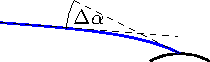
\includegraphics{licht/standalone/fig_delta_alpha.pdf}
  \caption{Skizze: Mass f"ur die Ablenkung $\Delta \alpha$. \label{fig:skizze_mass}}
\end{figure}

\section{Snelliussches Brechungsgesetz} 
\rhead{Snelliussches Brechungsgesetz}

Sehen wir am Ufer stehend einen Fisch im stillen Wasser eines Teiches, schwimmt er tats"achlich nicht genau an der vermuteten Stelle. 
Der Speer unserer Vorfahren w"urde ihn verfehlen, zielten sie direkt auf den Fisch.
Auf dem Weg vom Fisch zu unserem Auge durchbricht der Lichtstrahl den "Ubergang zwischen Wasser und Luft. 
Diese beiden Medien haben unterschiedliche Brechungsindizes $n_W$ und $n_L$, wodurch der Lichtstrahl an der Wasseroberfl"ache abgelenkt wird.
1621 fand auch der Mathematiker Snellius die nach ihm benannte zugrunde liegende Gesetzm"assigkeit:

\begin{equation} \label{eq:snellius}
n_W \cdot \sin \alpha_W = n_L \cdot \sin \alpha_L 
\end{equation}

In diesem einfachen Szenario setzen wir die Brechzahl $n(\vec{p}) = 1$ f"ur jeden Punkt im Wasser und in der Luft; nur genau an der Wasseroberfl"ache gilt $n(\vec{p}) = \frac{n_W}{n_L}$.
Wir stellen uns nun vor, dass wir statt einer einzigen Wasseroberfl"ache mehrere "ubereinander liegende Schichten von Medien verschiedener Brechungsindizes zwischen uns und dem Fisch sehen.
Weiter versetzen wir uns in die Lage des Fisches und beobachten die Speerspitze. 
Oder die eines Teleskops auf der Erdoberfl"ache welches auf Alpha Centauri gerichtet wird.

\section{Planares Modell} 
\rhead{Planares Modell}

Das planare Modell vernachl"assigt die Kr"ummung der Erdoberfl"ache und betrachtet die Atmosph"are als Abfolge von Luftschichten mit verschiedenen Brechungsindizes. 
Es ist schon intuitiv klar, dass diese Ann"ahrung nur f"ur steil nach oben gerichtete Teleskope aussagekr"aftig sein wird, wo aber auch die Ablenkung am kleinsten sein wird.
Wir verwenden ein 2-dimensionales kartesisches Koordinatensystem. 
Der Brechungsindex einer Luftschicht ist weiter nur von der H"ohe $y$ "uber Boden ab"angig und innerhalb einer Schicht konstant.

\begin{figure}
\centering
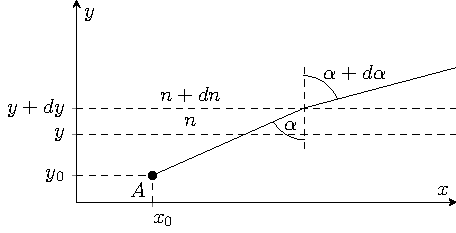
\includegraphics{licht/standalone/fig_planar_skizze.pdf}
\caption{Skizze des planaren Modells}
\label{fig:13_1}
\end{figure}

Wir m"ochten nun modellieren, dass es nicht einen haupts"achlichen, sondern viele kleine "Uberg"ange von einem Brechungsindex zum n"achsten gibt. 
Um nicht für jede Luftschicht eine neue Variable einzuf"uhren, dr"ucken wir den Brechungsindex der folgenden Luftschicht durch denjenigen der aktuellen Schicht plus eine kleine "Anderung aus. 
Gleiches setzen wir f"ur Ein- und Ausfallswinkel um. 
F"ur jeden "Ubergang zwischen zwei Luftschichten k"onnen wir somit das Brechungsgesetz wie folgt formulieren:

\begin{equation} \label{eq:13_1}
  n \cdot \sin(\alpha) = (n + dn) \cdot \sin(\alpha + d\alpha) = \text{const}
\end{equation}

Nun stellen wir den Weg des Lichstrahls mit $y(x_0) = y_0$ dar, wobei nun die Steigung $y'(x_0)$ der vertikalen Ausrichtung des Teleskops entspricht bzw. der Gegenwinkel von  $\alpha_0$ der H"ohe "uber dem Horizont.

Aus der Geometrie in der Abbildung \ref{fig:13_1} ist ersichtlich, dass wir mit 
$$\frac{\cos \alpha}{\sin \alpha} = \frac{dy}{dx} = y'(x)$$
einen Ausdruck für die Steigung dieser Funktion finden können. 
Wir haben damit die M"oglichkeit bekommen, folgende Umformung zu rechnen und anschliessend nach $\sin^2(\alpha)$ aufzul"osen.

$$ y'(x)^2 = \biggl(\frac{\cos \alpha}{\sin \alpha}\biggr)^2 = \frac{1 - \sin^2 \alpha}{\sin^2 \alpha} = \frac{1}{\sin^2 \alpha} - 1$$

\begin{equation} \label{eq:13_2}
\sin^2 (\alpha) = \frac{1}{y'(x)^2 + 1}
\end{equation}

Dies ist nicht ohne Division durch $(y'(x)^2 + 1)$ m"oglich, weshalb nun die Bedingung: ($y'(x)^2 +1) \neq 0$ gilt.
Als n"achstes quadrieren wir das angepasste Brechungsgesetz \ref{eq:13_1} und setzen \ref{eq:13_2} ein:
$$n^2 \cdot \frac{1}{y'(x)^2 + 1} = \text{const}^2 = (((n + dn)) \cdot \sin(\alpha + d\alpha))^2$$
Nun k"onnte man diese Gleichung numerisch l"osen. 
Wir m"ussen allerdings erst noch den Startwinkel $\alpha_0$ ber"ucksichtigen bzw. $y'(x_0)$.
Da in einer Differentialgleichung erster Ordnung die Steigung nicht Teil der Anfangsbedingung ist, leiten wir die Gleichung nach $x$ ab und erhalten:
$$\frac{d}{dx} \frac{n^2}{y'^2 + 1}  = \frac{2n}{y'^4 + 2y'^2 + 1} \cdot \left( n'(y'^2 + 1) - n y' y'' \right)$$
Die jetzt vorliegende Gleichung hat Ordnung 2 und der Anfangswinkel $\alpha_0$ ist nun Teil der Anfangsbedingung. 
Da $n(y)$ an allen Punkten abgesehen von den "Uberg"angen konstant ist, k"onnen wir $0$ setzen.
Somit muss der Ausdruck in den Klammern ebenfalls gleich $0$ sein.
Da sich $n$ nur in y Richtung "andert bzw. $\frac{dn}{dx} = \frac{dn}{dy} \cdot \frac{dy}{dx}$, wird im Folgenden die Notation $n'_y = \frac{dn}{dy}$ verwendet.
$$0 = n' y'^2 + n' - n y' y''$$
$$y''(x) = \frac{n'_y}{n} \cdot \left( y' + \frac{1}{y'} \right)$$
\begin{equation} \label{eq:planar_DGL}
y''(x) = \frac{n'_y}{n} \cdot \left( y'^2 + 1\right)
\end{equation}

\subsection{Verifikation}
Um zu "uberpr"ufen, ob unser Modell plausibel ist, setzen wir verschiedene Funktionen f"ur $n(y)$ ein. 
Wenn die Brechzahl konstant ist (also $\frac{dn}{dy} = 0$), dann sollte der Lichtstrahl nicht mehr gebrochen werden und auf einer Geraden weiterfahren. 
Wenn man nun $n'(y)=0$ in die Gleichung \ref{eq:planar_DGL} einsetzt, erh"alt man: 
$$y''(x) = 0$$
Auch aus unserer Gleichung ist also erkennbar, dass sich der Lichtstrahl bei konstantem $n$ nicht bricht.
Nun brauchen wir eine Funktion der Brechzahl in Abh"angigkeit der H"ohe. 
Der Brechungsindex der Luft h"angt unter anderem vom Luftdruck ab. 
Dieser nimmt nach der barometrischen H"ohenformel mit der H"ohe exponentiell ab.
Ausserdem ist die Brechzahl immer $n \geq 1$, wobei im Vakuum $n=1$ gilt. 
Mit diesen Informationen stellen wir eine modellierung der Brechzahl folgendermassen zusammen:
$$n(y) = 1 + \mu e^{- \sigma y}, \qquad \frac{dn}{dy} = -\sigma \mu \cdot e^{-\sigma y}$$
Nun setzen wir dies in die Differentialgleichung ein, und erhalten:
\begin{equation} \label{eq:planar_DGL_n}
y''(x) = \frac{-\sigma}{\displaystyle\frac{1}{\mu e^{-\sigma y}} + 1} \cdot \left( y'^2 + 1 \right)
\end{equation}
Wie man anhand der Vorzeichen in \ref{eq:planar_DGL} erkennen kann, kr"ummt sich der Lichstrahl immer in Richtung des gr"osseren $n$.
Bei dem von uns verwendeten $n(y)$ bedeutet dies, dass er sich nach unten kr"ummt. 
Um dies besser darzustellen, wird die Brechzahl in den Grafiken grau eingezeichnet.
Diese Differentialgleichung l"asst sich numerisch l"osen (siehe Abbildung \ref{fig:planares_modell1}).
Die modellierte Brechzahl wurde in dieser Abbildung in grau dargestellt. 
Die Ableitung von $f$ an der Stelle $0$ modelliert dabei die H"ohe "uber dem Horizont.
Wie zu erwarten war, kr"ummen sich die Lichtstrahlen nach unten.
Je steiler der Strahl ist, desto schw"acher kr"ummt er sich. 
\begin{figure}
  \centering
  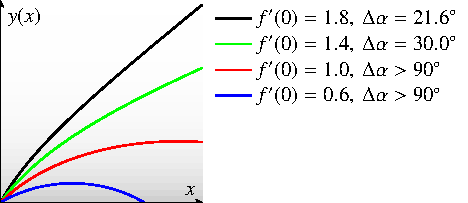
\includegraphics{licht/standalone/fig_planar_simulation.pdf}
  \caption{Numerische L"osung der Differentialgleichung (\ref{eq:planar_DGL_n}). \label{fig:planares_modell1}}
\end{figure}

% Vorschlag: 
% Diesen Unterabsatz komplett Auslassen.
% 
\subsection{Spezialfall: Lichtstrahl parallel einer konstanten H"ohe \label{ch:spezialfall}}
In diesem Modell ist die Brechzahl $n$ nur von $y$ abh"angig. 
Falls die Funktion nun die Steigung $y'(x) = 0$ hat, dann "andert sich die Brechzahl in Richtung des Lichtstrahls nicht mehr.
Dies w"urde bedeuten, dass sich der Lichtstrahl nicht weiter kr"ummt. 
In der Realit"at gibt es in der Luft immer relativ starke Unregelm"assigkeiten. 
Betrachten wir das Beispiel der Abbildung \ref{fig:planares_modell1}. 
Falls der Lichtstrahl waagerecht ist, kann er aufgrund diese Unregelm"assigkeiten entweder nach oben oder unten gebrochen werden. 
In der Realit"at ist dieser Spezialfall also nicht allzuh"aufig anzutreffen.

\subsection{Fazit planares Modell}
Wir haben mit dem planaren Modell eine erste Modellierung einer kontinuierlichen Brechzahl simulieren k"onnen und sind mit den Resultaten qualitativ zufrieden. 
Entgegen der Meinung gewisser Minderheiten\cite{licht:flatearthsociety} leben wir aber auf einem kugelf"ormigen Planeten, weshalb wir nun eine sph"arische Geometrie aufbauen m"ochten.

\section{Sph"arisches Modell}
\rhead{Sph"arisches Modell}

Anstatt "ubereinanderliegender Luftschichten betrachten wir nun ineinanderliegende Sph"ahren mit konstantem Innen- und Aussenradius.
Weiterhin nehmen wir an, dass $n$ nur von der H"ohe "uber dem Boden abh"angt bzw. $n(r)$ und die geografische L"ange oder Breite des Teleskops keinen Einfluss auf $n$ haben.
So richten wir ein 2-dimensionales, polares Koordinatensystem so aus, dass das Teleskop auf $(r = r_0, \varphi=0)$ zu stehen kommt.
Wir beginnen erneut mit dem Brechnungsgesetz von Snellius, welche wir auf unser sph"arisches Modell (Abbildung \ref{fig:sphere_skizze}) angepassen: 
\begin{equation} \label{eq:snellius_spheric}
n \cdot \sin \beta = (n + dn) \cdot \sin(\alpha + d\alpha)
\end{equation}
In dieser Gleichung kommen zwei verschiedene Winkel $\alpha$ und $\beta$ vor. 
Um dies zu bereinigen verwenden wir den Sinussatz im Dreieck $OMN$
\footnote{Verl"angert man $\overline{MN}$ nach unten und f"allt darauf ein Lot durch $O$ kann Gleichung \ref{eq:snellius_spheric} direkt im entstehenden rechtwickligen Dreieck abgelesen werden, wenn man die L"ange der gemeinsamen Gegenkathete der beiden Sinusterme gleichsetzt.}:
\begin{equation} \label{eq:snellius_spheric2}
r \sin\alpha = (r + dr) \cdot \sin\beta
\end{equation}
Multipliziert man nun die beiden Gleichungen, erh"alt man:
\begin{equation} \label{eq:sphere_base}
n r \sin \alpha = (n + dn)(r + dr) \sin (\alpha + d\alpha) = n_0 r_0 \sin \alpha_0
\end{equation}
Somit sind nicht mehr zwei verschiedene Winkel in der Formel vorhanden.
Wie beim planaren Modell ist dieses Produkt konstant.  
Aus dem Dreieck $MNP$ kann folgende Beziehung hergeleitet werden:
$$\tan \alpha =  \frac{\overline{NP}}{\overline{MP}} = \frac{r \cdot d\varphi}{dr} = \frac{r}{r'}$$
Wir quadrieren die Gleichung und l"osen nach $\sin^2(\alpha)$ auf:
$$\tan^2 \alpha = \frac{\sin^2\alpha}{\cos^2\alpha} = \frac{\sin^2\alpha}{1-\sin^2\alpha} = \frac{1}{\displaystyle\frac{1}{\sin^2\alpha}-1} = \left( \frac{r}{r'} \right)^2$$
\begin{equation} \label{eq:sphere_sine}
\Rightarrow \sin^2\alpha = \frac{1}{\left( \frac{r'}{r} \right)^2 +1}
\end{equation}
\begin{figure} 
\centering
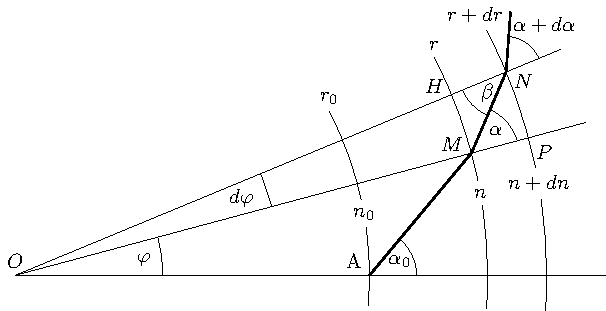
\includegraphics[scale=1]{licht/standalone/fig_sphere_skizze.pdf}
\caption{Skizze des sph"arischen Modells. \label{fig:sphere_skizze}}
\end{figure}
W"ahrend diesen Umformungen wurde durch $r'(\varphi)$ geteilt. 
In den folgenden Gleichungen sei Vorausgesetzt, dass $r'(\varphi) \neq 0$. 
Wie bereits zuvor in Kapitel \ref{ch:spezialfall} beschrieben muss dieser nicht separat behandelt werden.
Nun quadrieren wir die Gleichung (\ref{eq:sphere_base}) und setzen die Gleichung (\ref{eq:sphere_sine}) ein:
$$\frac{(n \cdot r)^2}{\displaystyle\left( \frac{r'}{r} \right)^2 +1} = (r_0 n_0 \sin \alpha_0)^2$$
Diese Gleichung ist eine Differentialgleichung erster Ordnung. 
Jedoch ist erneut der Term $\sin^2(\alpha_0)$ vorhanden, welcher von $r'(0)$ abh"angt. 
Damit die DGL auch korrekte Anfangsbedingungen besitzt, leiten wir die Gleichung nach $\varphi$ ab und erhalten:

\begin{equation}
\begin{aligned}
\frac{d}{d\varphi}\frac{(n r)^2}{\left(\displaystyle\frac{r'}{r}\right)^2 + 1} 
& = \frac{2 r^2 n r' n'_r}{\displaystyle\frac{r'^2}{r^2}+1}+\frac{2 r n^2 r'}{\displaystyle\frac{r'^2}{r^2}+1}-\frac{r^2 n^2 \left(\displaystyle\frac{2 r' r''}{r^2}-\frac{2 r'^3}{r^3}\right)}{\left(\displaystyle\frac{r'^2}{r^2}+1\right)^2} \\
& = \frac{2n r' r}{\displaystyle\frac{r'^2}{r^2}+1} \cdot \left( n'_r + n - \frac{n r r'' - n r'^2}{r'^2 + r^2} \right)
\end{aligned}
\end{equation}
Wie beim planaren Modell k"onnen wir auch hier die zweite Ableitung Null setzen, um einen Ausdruck f"ur $r''$ zu erhalten.
\begin{equation}
\Rightarrow n'_r + n - \frac{n r r'' - n r'^2}{r'^2 + r^2} = 0
\end{equation}
$$\Rightarrow n'_r r'^2  + n'_r r^2 + n r'^2 + nr^2 = n r r'' - n r'^2$$
$$\Rightarrow n'_r r'^2 + n'_r r^2 + 2 n r'^2 + n r^2 = n r r''$$
\begin{equation} \label{eq:sphere_allg}
\Rightarrow r'' = \frac{n'_r r'^2 + n'_r r^2 + 2 n r'^2 + n r^2}{n r}
\end{equation}
Anmerkung: Da $\frac{dn}{d\varphi} = \frac{dn}{dr} \cdot \frac{dr}{d\varphi}$ ist, wird die Notation: $n'_r = \frac{dn}{dr}$ verwendet.

\subsection{Verifikation}
Wie zuvor beim planaren Modell setzen wir verschiedene Funtionen f"ur $n(r)$ ein, und beurteilen die Resultate. 
Als erstes untersuchen wir die Funktion $n(r) = 1, n'(r) = 0$. 
Bei diesem Beispiel hat das Material "uberall dieselbe Brechzahl.
Die numerischen L"osungen sollten alle (bez"uglich den kartesischen Koordinaten) linear ansteigen und sich nicht kr"ummen. Die Simulation best"atigt dies (siehe Abbildung \ref{fig:sphaerisches_modell1}).

Nun verwenden wir erneut die exponentielle Approximation der Brechzahl: 

$$n(r) = 1 + \mu \cdot e^{-\sigma (r - r_0)}, \qquad n'_r(r) = -\sigma \mu e^{-\sigma (r - r_0)}$$

Nun setzen wir dies in die Differentialgleichung (\ref{eq:sphere_allg}) ein und berechnen die L"osung numerisch (Abbildung \ref{fig:sphaerisches_modell2}, \ref{fig:sphaerisches_modell3}). 

\begin{figure}
\centering
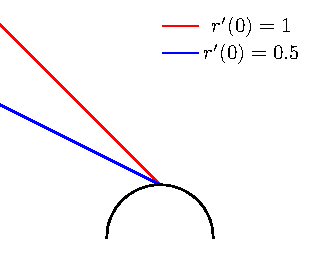
\includegraphics[scale=1]{licht/standalone/fig_sphere_simulation_vacuum.pdf}
\captionof{figure}{L"osung des sph"arischen Modells mit $n(r) = 1$. \label{fig:sphaerisches_modell1}}
\end{figure}

\begin{figure}
\centering
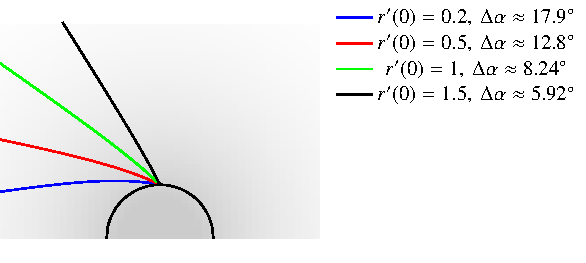
\includegraphics[scale=1]{licht/standalone/fig_sphere_simulation1.pdf}
\caption{Numerische L"osung der Exponentiellen Approximation mit $\mu = 1, \: \sigma = 0.5$. 
\label{fig:sphaerisches_modell2}}
\end{figure}

\begin{figure}
\centering
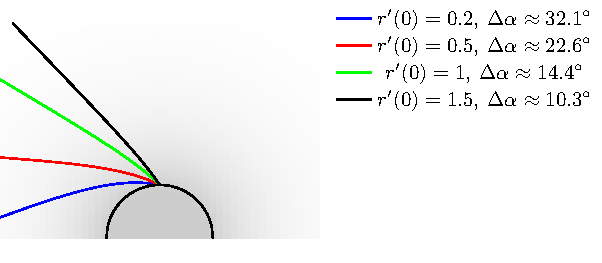
\includegraphics[scale=1]{licht/standalone/fig_sphere_simulation2.pdf}
\caption{Numerische L"osung der Exponentiellen Approximation mit $\mu = 1, \: \sigma = 1$. \label{fig:sphaerisches_modell3} }
\end{figure}

\newpage

\subsection{Spezialfall: Geschlossener Kreis}
Beim Betrachten der Resultate f"allt auf, dass es m"oglicherweise eine Kombination aus Anfangsbedingungen und der Brechzahl gibt, welche das Licht in einem Kreis um den Planeten bricht. 
Um diese Bedingungen zu finden, starten wir mit der Gleichung \ref{eq:sphere_origin}:
$$\Rightarrow n'_r + n - \frac{n r r'' - n r'^2}{r'^2 + r^2} = 0$$
Bei diesem Spezialfall ist $r''(\varphi) = 0$, $r'(\varphi) = 0$. 
Setzen wir nun diese Bedingungen in die Gleichung ein, erhalten wir:
$$n'_r + n = 0 \quad \Rightarrow \quad n'_r(r) = -n(r)$$
Dies ist nun ebenfalls eine Differentialgleichung, welche die L"osung $n(r) = C \cdot e^{-r}$ hat.
Alle diese L"osungen haben die Eigenschaft, dass man bei dieser Verteilung der Brechzahl ein waagerechter Lichtstrahl auf jeder H"ohe in einen geschlossenen Kreis gebrochen wird.
Da diese L"osung die Bedingung $n(r) \geq 1$ jedoch nicht erf"ullt, gibt es keine m"ogliche Verteilung der Brechzahlen, bei der auf jeder H"ohe der waagrechte Lichtstrahl zu einem Kreis gebrochen wird. 
Jedoch ist es m"oglich, dass diese Bedingung auf genau einer H"ohe zutrifft. 
Dieser Effekt erlangte im sp"aten 19. Jahrhundert tragisch-komische Ber"uhmtheit, als Samuel Rowbotham durch seine Beobachtungen zum Schluss kam, dass die Erde flach sein muss. 
Das Weltbild bereits genannter Minderheit\cite{licht:flatearthsociety} unserer Gesellschaft geht auf diesen Irrtum zur"uck. Doch was steckt dahinter? 
Wir untersuchen wieder die exponentielle Approximation mit:
$$n(r) = 1 + \mu \cdot e^{-\sigma (r-r_0)} \qquad n'(r) = -\mu \sigma \cdot e^{-\sigma (r-r_0)}$$
Wir setzen diese Funktionen nun in die obige Bedingung ein und erhalten:
$$\mu \sigma \cdot e^{-\sigma (r-r_0)} = 1 + \mu \cdot e^{-\sigma (r-r_0)} \quad \\
\Rightarrow \quad \mu \cdot e^{-\sigma (r-r_0)} \cdot (\sigma - 1) = 1 \\
\Rightarrow \mu = \frac{e^{\sigma (r-r_0)}}{\sigma - 1}$$
Wenn wir $r = r_0$ und $\sigma = 2$ festhalten, ergibt sich $\mu = 1$. 
Auch die Simulation best"atigt, dass in diesem Fall das Licht in einem Kreis gebrochen wird.
In der Simulation wurde auch ein leicht verf"alschter Lichtstrahl dargestellt, mit 0.01 Abweichung. 
Da es in der Luft immer viele Unregelm"assigkeiten des Druckes, der Temperatur und der Luftfeuchtigkeit gibt, soll dieser Lichtstrahl zeigen, wie sich ein solcher Fehler auf den Verlauf auswirkt.
Wie man erkennen kann ist dieser Lichtstrahl bis $90^\circ$ nicht vom anderen zu unterscheiden.
Bei der Simulation ist jedoch der Radius mit $r_0=1$ sehr klein gew"ahlt worden. 
Wenn der Radius gr"osser gemacht wird ($r_0 = 100$), so  verl"asst der Lichtstrahl viel fr"uher den pfad (Abbildung \ref{fig:sphere_special2}). 
Jedoch ist eine solch extreme Atmosph"are nicht realistisch. 
Bei $r = r_0$ betr"agt die Brechzahl $n(r_0) = 1 + \mu = 2$. 
Diese Brechzahl ist nicht realistisch. 
Es braucht also ein anderes Modell, mit dem man diesen Effekt erzeugen kann.
Die Brechzahl der Luft ist nicht nur vom Druck abh"angig, sondern auch von der Luftfeuchtigkeit. 
dazu wird folgende quadratische Approximation verwendet:
$$n(r) = \left\{ \begin{array}{ll} 1 + \mu \cdot (r_0 - r)^2 & \text{wenn } r < r_0 \\ 1 & \text{sonst} \end{array} \right. \quad n'_r(r) = \left\{ \begin{array}{ll} 2\mu \cdot (r - r_0) & \text{wenn } r < r_0 \\ 0 & \text{sonst} \end{array} \right.$$
Nun l"osen wir die obere Bedingung $-n'_r = n $, wenn $r < r_0$:
$$2\mu \cdot (r_0 - r) = 1 + \mu(r_0 - r)^2$$
Wenn wir nun f"ur $(r_0 - r) = 1$ einsetzen, erhalten wir $\mu = 1$. 
Bei der Simulation mit diesen Bedingungen ist ersichtlich, dass in einen Kreis gebrochen wird (Abbildung \ref{fig:sphere_special3}). 
Wenn aber wie erneut der Fehler Simuliert wird, ist die Abweichung viel kleiner als bei der exponentiellen Approximation. 
Nun erh"ohen wir ebenfalls den Radius $r_0$ und wiederholen die Simulation. 
Bei $r_0 = 1000$ ist der Lichtstrahl immer noch f"ur lange Zeit auf dem idealen Kreis (Abbildung \ref{fig:sphere_special4}). 
Bei dieser Approximation ist es also m"oglich, dass sich ein Lichtstrahl f"ur kurze Zeit in einen Kreisbogen bricht, auch bei gr"osserem $r_0$.
\begin{figure}
  \centering
  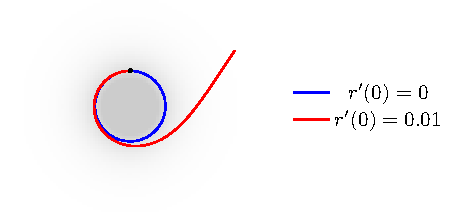
\includegraphics[scale=1]{licht/standalone/fig_kreis_exp1.pdf} 
  \caption{Numersiche L"osung der exponentiellen Approximation mit $r(0) = r_0 = 1$, $r'(0) = 0$, $\sigma = 2$, $\mu = 1$. \label{fig:sphere_special1}}

\end{figure}

\begin{figure}
  \centering
  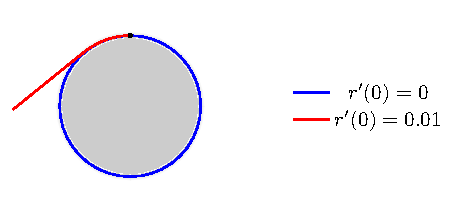
\includegraphics[scale=1]{licht/standalone/fig_kreis_exp2.pdf}
  \caption{Numerische L"osung der exponentielle Approximation mit $r(0) = r_0 = 100$, $\sigma = 2$, $\mu = 1$. \label{fig:sphere_special2}} 
  
\end{figure}

\begin{figure}
  \centering
  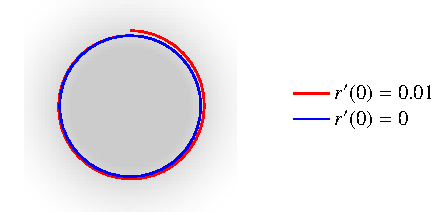
\includegraphics[scale=1]{licht/standalone/fig_kreis_square1.pdf}
  \caption{Numerische L"osung der quadratischen Approximation mit $r(0) = r_0 = 1$, $mu = 1$. \label{fig:sphere_special3} }
  
\end{figure}

\begin{figure}
  \centering
  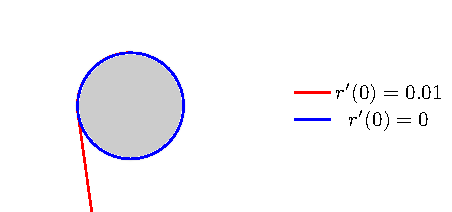
\includegraphics[scale=1]{licht/standalone/fig_kreis_square2.pdf}
  \caption{Numerische L"osung der quadratischen Approximation mit $r(0) = r_0 = 1000$,  $\mu = 1$. \label{fig:sphere_special4} } 
\end{figure}

\section{Modellierung der Atmosph"are der Erde}
\rhead{Modellierung der Atmosph"are der Erde}

Bei bisherigen Simulationen sind wir von einer (willk"urlichen) Funktion ausgegangen, ohne uns dabei auf reale Daten zu st"utzen. 
Nun wollen wir ein m"oglichst realistisches, aber dennoch einfaches Modell f"ur die Atmosph"are der Erde finden.
Die Brechzahl der Luft h"angt von folgenden Faktoren ab:
\begin{itemize}
  \item Wellenl"ange des Lichts: In unserem Modell gehen wir von einer konstanten Wellenl"ange aus. Dieser Effekt wird nicht ber"ucksichtigt.
  \item Wasserfeuchtigkeit: Wasserdampf Anteil in der Luft beeinflusst die Brechzahl relativ stark. Jedoch variiert diese sehr stark mit dem Wetter. Deshalb wird dieser Einfluss vernachl"assigt. 
  \item Luftdruck: Der Luftdruck l"asst sich approximativ relativ gut modellieren. Aus der Physik ist bekannt, dass der Druck bei Gasen mit der H"ohe exponentiell abnimmt. 
  \item Temperatur: Wie in Abbildung \ref{fig:athmosphere_profile} erkennbar ist, ver"andert sich die Temperatur in abh"angigkeit der H"ohe sehr stark. Es ist jedoch sehr schwer, diesen Verlauf zu modellieren. Deshalb wird die Temperatur (vorerst) im Modell vernachl"assigt.
\end{itemize}

\begin{figure}
  \centering
  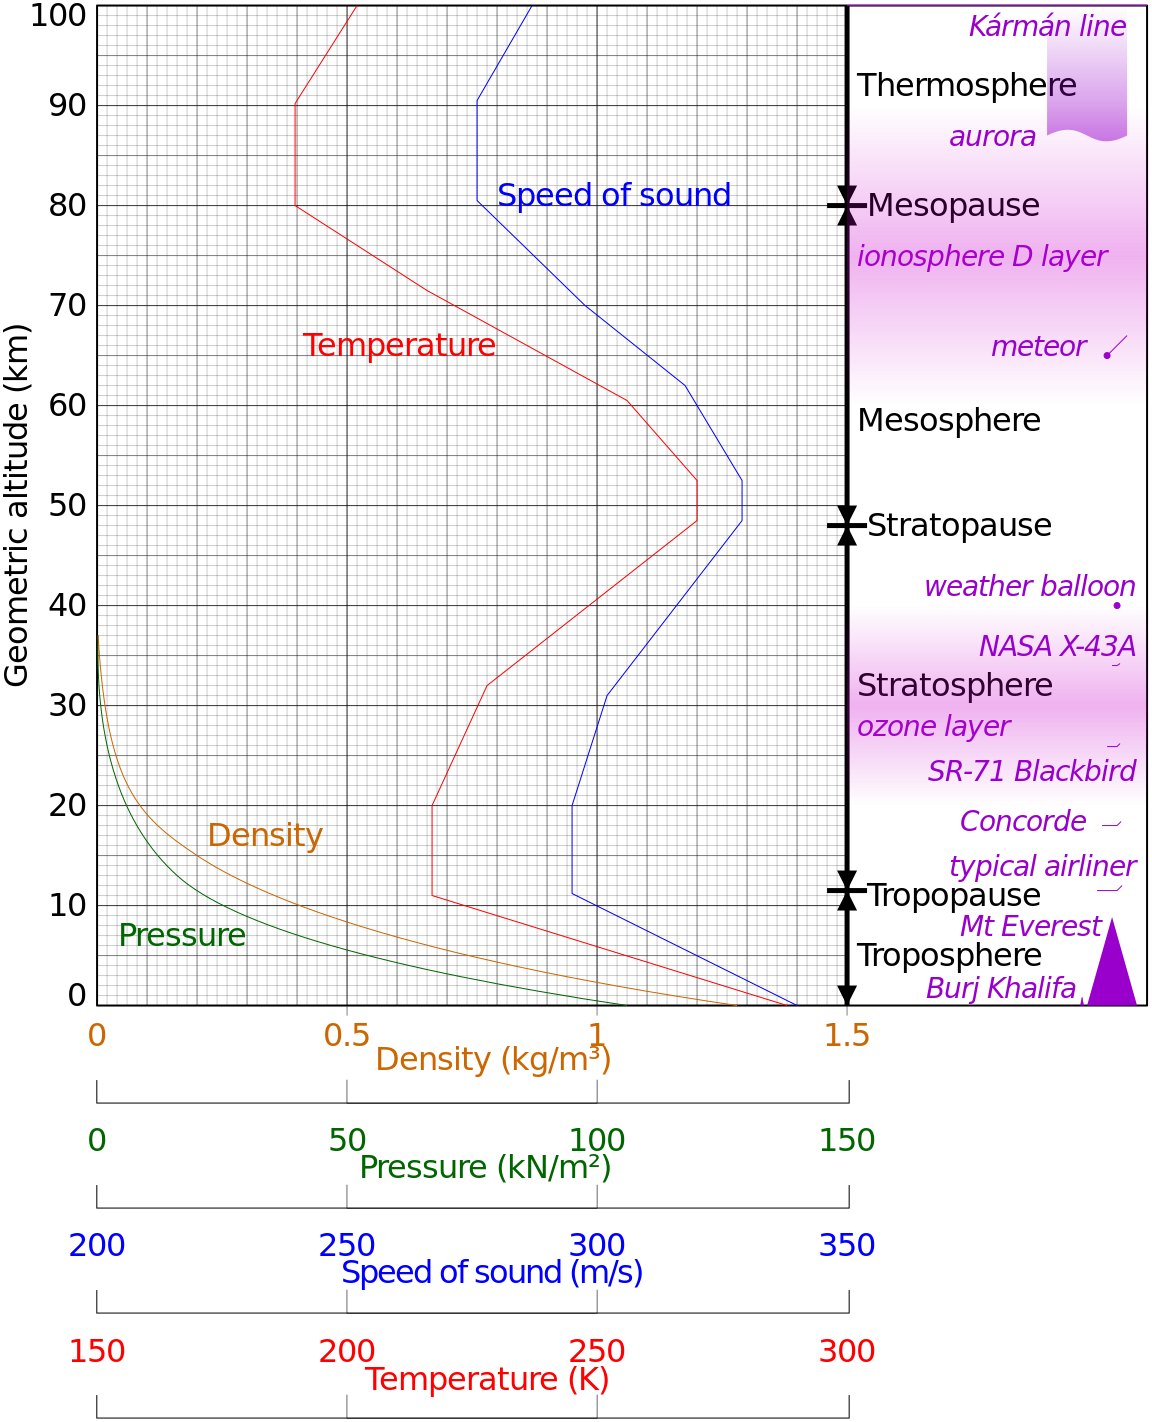
\includegraphics[scale=0.24]{licht/images/athmosphereProfile.png}
  
  \caption{Druck, Dichte, Temperatur und Schallgeschwindigkeit in Abh"angigkeit der H"ohe. \label{fig:athmosphere_profile}}
\end{figure}

Dank diesen Vereinfachungen l"asst sich die Brechzahl in Abh"angigkeit folgendermassen beschreiben:
$$n(r) = 1 + \mu \cdot e^{-\sigma (r - r_0)}$$
Der Parameter $r_0$ steht f"ur den Radius der Erdoberfl"ache. 
Bei $r = r_0$ ergibt sich $n(r_0) = n_0 = 1 + \mu$. 
$\sigma$ gibt an, wie schnell die Brechzahl zum tiefsten Wert $n = 1$ geht. 
Durch Messungen ist der mittlere Erdradius $r_0 = 6.371 \cdot 10^6$. 
Die Brechzahl auf dieser H"ohe betr"agt: $n_0 = 1.000293$.
Dementsprechend betr"agt $\mu = 2.93 \cdot 10^{-3}$. 
Um $\sigma$ abzusch"atzen, wird in der Abbildung \ref{fig:athmosphere_profile} Funktion der Dichte untersucht. 
Die H"ohe bei 36.8\% der Maximaldichte (Dichte auf Meeresh"ohe) entspricht $\sigma$. 
Somit wird $\sigma \approx 9 \cdot 10^3$.
Mit diesen Parametern l"asst sich die erneut die L"osung zum sph"arischen Modell numerisch berechnen. 
Aufgrund der Parameter erwarten wir eine sehr schwache Kr"ummung. 
Dies kann man auch an der Abbildung \ref{fig:sphere_real} erkennen. 
Die Vergleichsgr"osse $\Delta \alpha$, welche aus der Simulation resultiert, zeigt erneut, dass der Lichtstrahl st"arker gebrochen wird, wenn er horizontal eintrifft. 

\begin{figure}
  \centering
  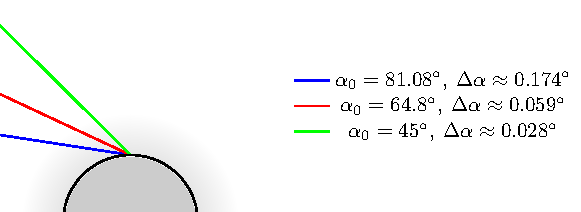
\includegraphics[scale=1]{licht/standalone/fig_real_simulation.pdf}
  \caption{Numerische L"osung des realistischen Modells. \label{fig:sphere_real} } 
\end{figure}

\begin{figure}
  \centering
  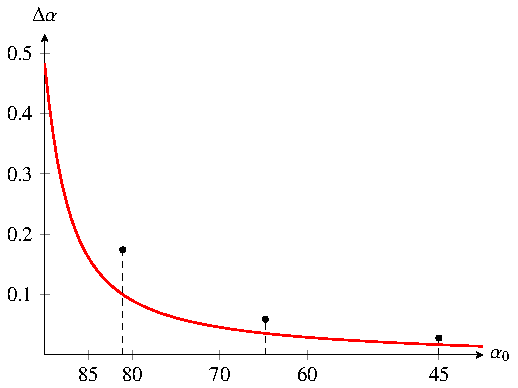
\includegraphics[scale=1]{licht/standalone/fig_real_comparison.pdf}
  \caption{In der Praxis genutzte Approximationskurve f"ur verglichen mit den Simulationsergebnissen. \label{fig:real_comparison}}
\end{figure}

\section{Fazit und Zusammenfassung}
\rhead{Fazit und Zusammenfassung}
Basierend auf dem Brechungsgesetz von Snellius haben wir uns 2 verschiedene Geometrien angesehen und verschiedene Modellierungen der Brechzahl darin simuliert und numerisch ausgewertet. 
Die Ergebnisse liegen erfreulich nahe an den in der Praxis zur Bereinigung benutzten Werte.
Die mathematischen Eigenschaften der verwendeten Gleichungen, zeigen erste Grenzf"alle an, welche tats"achlich auch besonderen Sitationen in der Natur entsprechen.

\printbibliography[heading=subbibliography]
\end{refsection}